\documentclass{article}

\usepackage{algorithmic}
\usepackage{amsmath}
\usepackage{graphicx}

\begin{document}

\title{Bayesian Particle Filter Tracking with CUDA}
\author{Geoffrey Ulman\\
        CSI702}
\date{April 2010}
\maketitle

\tableofcontents

\section{Introduction}\label{Introduction}
Bayesian particle filtering techniques provide a flexible toolkit for solving a wide array of data fusion problems. This paper uses a specific motivating example to explore how effectively Bayesian particle filtering can be adapted to CUDA.

The motivating problem is as follows: A submarine with a hydrophone (passive sonar) is following another ship and attempting to estimate that ship's location and speed using the direction of the sound from the ship's engine as recored by the hydrophone. However, the hydrophone is imperfect and the observed direction of the sound does not exactly correspond to the true location of the ship. How can these errored bearing observations be used to develop an estimate of the ship's true position and velocity?

\section{Background}\label{Background}
At its core, Bayesian particle filtering is an iterative process by which a collection of particles approximating a probability distribution are updated based on incoming data to better approximate the true state of a target being observed.

Each particle represents a possible target state and the collection of particles approximates a probability distribution, called a prior, which describes the possible states of the target (see Section \ref{Prior Distribution}). When a new observation arrives, the particles are time updated to reflect the time of the observation. Then, a likelihood function (see Section \ref{Likelihood Functions}) is used to updated the weights of the particles based on the new information contained in the observation. Finally, resampling is performed to replace low weight particles with randomly perturbed copies of high weight particles (see Section \ref{Resampling}).

\subsection{Prior Distribution}\label{Prior Distribution}
Employing Bayesian tracking to estimate the true state \(x\) of a target in a state space \(S\) requires starting with a probability density function \(p(x)\) which is referred to as the prior distribution. The prior is a probability density function over the state space \(S\) which gives the probability that any given \(x \in S\) is the true target state. Because the prior must be provided before any observations are received, it is generally based on engineering knowledge of the targets and of the sensors used to generate observations.

For example, the state space for the submarine tracking problem considered here is four-dimensional, consisting of two Cartesian position dimensions and two velocity dimensions. A simple uniform bounded distribution on the two position and two velocity state space dimensions is used as the prior (reflecting that we know very little initially about the true target state). Figure \ref{prior} displays the \(x\) and \(y\) position components of the prior. Because all particles are initially weighted equally, any particle has an equal likelihood of being the true state of the target.

\begin{figure}
\centering
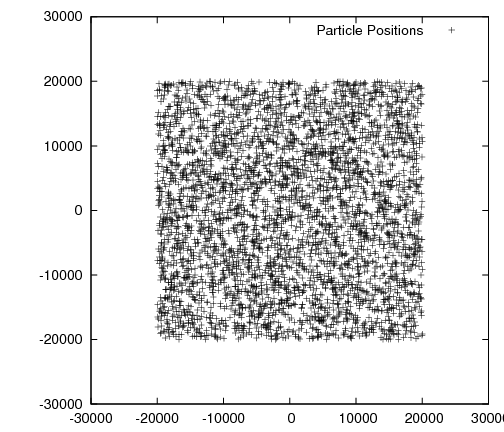
\includegraphics[width=0.7\textwidth]{data/particles_prior.png}
\caption{Prior Particle Position Distribution}
\label{prior}
\end{figure}

\subsection{Likelihood Functions}\label{Likelihood Functions}
Equation \ref{lfunc1} describes a likelihood function \(L\) for observation \(Y=y\) and random variable \(X\) which takes on values in a state space \(S\). The function \(P(\cdot|x)\) is a probability density function describing the probability of obtaining observations \(y\) from the sensor given a known target state \(x\).

However, in Bayesian tracking, the function \(P(y|\cdot)\) is far more interesting. In tracking problems, observations \(y\) are fixed and the true target state \(x\) is unknown. When viewed as a function of \(x\), we call \(P(y|\cdot)\) a likelihood function. The likelihood function can be used in conjunction with Bayes' rule to modify our prior distribution \(p(x)\) (discussed in Section \ref{Background}) to incorporate the information from an observation \(y\).

The name likelihood function arises from the fact that for \(x_{1},x_{2} \in S\), if \(L(y|x_{1})>L(y|x_{2})\), then the observation \(y\) is more likely to have come from a target with state \(x_{1}\) than a target with state \(x_{2}\). Is should also be noted that unlike \(P(\cdot|x)\), the likelihood function is usually not a probability density function.\cite{bmtt}

\begin{equation}\label{lfunc1}
L(y|x) = P( Y=y | X=x ) \verb! for ! x \in S
\end{equation}

Once we have the notion of a likelihood function, we can write Equation \ref{lfunc2} which is the core of Baysian tracking. It describes how to modify the prior \(P(x)\) to reflect the addition of the new information contained in the observation \(y\) and obtain a posterior distribution \(P(x|y)\). This posterior distribution can have further likelihood functions applied to it using Equation \ref{lfunc2} to incorporate additional information. This iterative process is known as Bayesian tracking.

Particle filtering provides a convenient way to perform the calculations described by Equation \ref{lfunc2}. The likelihood function is evaluated for each particle and the result is multiplied by that particle's weight to obtain an updated weight. The updated particle weights are then normalized by the sum over all particle weights to obtain the posterior distribution.

\begin{equation}\label{lfunc2}
P(x|y) = \frac{L(y|x)P(x)}{\int \! L(y|x)P(x) \, dx}
\end{equation}

Figure \ref{posterior1} shows the posterior distribution after the likelihood for a single azimuth observation is applied to the prior distribution from Figure \ref{prior}. An azimuth observation is a single angle value indicating that the target is somewhere along the ray starting at the sensor's current position and continuing in the given angle. The likelihood function which we associate with such observations, shown in Equation \ref{lfunc3}, is a simple Gaussian distribution in azimuth space.\cite{bmtt}

In Equation \ref{lfunc3}, \(\theta\) is an azimuth observation, \(x \in S\) is an element of the state space, \(\sigma\) is the standard deviation assigned to the observation, and \(b(\alpha,x)\) is a function which gives the azimuth from the sensor position \(\alpha\) to the position \(x\).

\begin{equation}\label{lfunc3}
L(\theta|x)=(2\pi\sigma^{2})^{\frac{-1}{2}}e^{\frac{-(\theta-b(\alpha,x))^{2}}{2\sigma^{2}}}
\end{equation}

\begin{figure}
\centering
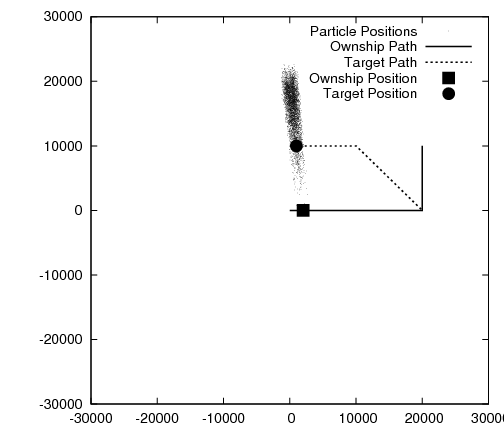
\includegraphics[width=0.7\textwidth]{data/particles_azimuth_obs.png}
\caption{Posterior Particle Position Distribution after Azimuth Observation}
\label{posterior1}
\end{figure}

\subsection{Motion Model}
In kinematic tracking problems observations often occur at different times. The existence of velocity components in the state space \(S\) indicates that the position components are changing over time. In addition, the possibility that the target might change its velocity must be modeled.

Motion updating can be described much more generally and rigorously, but in our case the step is simple. Particles make instantaneous velocity adjustments with an exponentially distributed mean time between adjustments. During periods where no adjustment is made, particles travel at a constant velocity. If no observations are received for an extended period of time, as has happened in Figure \ref{posterior2}, the particles will drift apart on their constant velocity paths and the posterior distribution will become more diffuse to indicate our increasing uncertainty about the current location of the target.

\begin{figure}
\centering
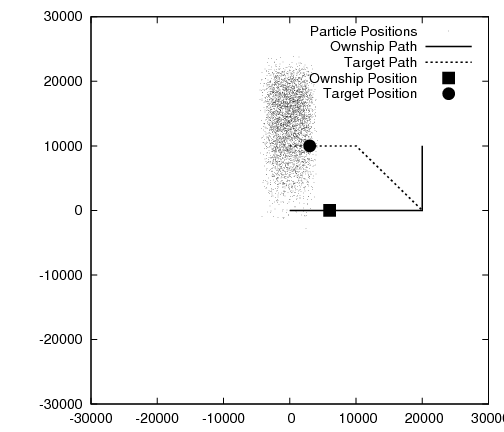
\includegraphics[width=0.7\textwidth]{data/particles_motion.png}
\caption{Posterior Particle Position Distribution after Azimuth Observation and Motion Update}
\label{posterior2}
\end{figure}

\section{Design}
Most portions of the Bayesian tracking recursion are embarrassingly parallel operations which map directly to CUDA without much trouble. Initialization of particle positions, time updating, and information updating are all performed on each particle individually. However, the CUDA implementation other portions of the algorithm, including resampling and random number generation, provide interesting challenges.

\subsection{Resampling}\label{Resampling}
As observations containing information about the target's state are incorporated into the prior distribution using appropriate likelihood functions, some particles will match very poorly with the observations and receive low weight as a result. Eventually, keeping such particles around serves very little purpose, since the Bayesian tracker has already indicated that they match poorly with the observations and are thus unlikely to represent the true target state. Resampling is a technique for remedying this situation by periodically replacing particles with low weight with slightly perturbed copies of particles with high weight.

\subsubsection{First Resampling Implementation}

\[ C = \frac{n}{\sum_{i=0}^{n} w_{i}} \]
\begin{equation}\label{resample1}
\overline{w}_{i}=C w_{i}
\end{equation}

\begin{equation}\label{resample2}
\hat{w}_{i}=\operatorname{floor}(\sum_{j=0}^{i} \overline{w}_{j})
\end{equation}

When copying particles, we want each particle to have a likelihood of being copied proportional to its weight. Equation \ref{resample1} describes the transformation applied to particle weights \(w_{i}\) to obtain the number of copies to make of each particle. However, to implement the copy operation in parallel in CUDA, each particle must also know where in global memory its copies should be placed.

Equation \ref{resample2} solves this problem by calculating a cumulative sum of weights. With the cumulative sum in hand, thread \(i\) simply makes \(\hat{w}_{i}-\hat{w}_{i-1}\) copies of the particle at index \(i\) and places them in the contiguous block of memory from \(\hat{w}_{i-1}\) to \(\hat{w}_{i}\).

\begin{figure}
\centering
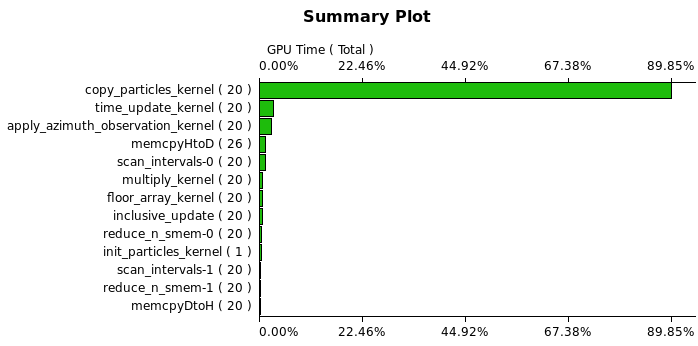
\includegraphics[width=0.7\textwidth]{data/profile_cuda_version1_pic1.png}
\caption{CUDA Visual Profiler Version 1 Results}
\label{profiler1}
\end{figure}

Unfortunately, as indicated by Figure \ref{profiler1}, this approach is very slow on GPU hardware because of the large amount of uncoalesced memory access which it must perform. Further, most threads sit idle (those with low enough weights that they make 0 copies of themselves) while a very few perform all the memory copies.

\subsubsection{Second Resampling Implementation}\label{resamplesection2}

The second resampling algorithm implementation improves on the first dividing the work of duplicating particles more evenly among the threads. Instead of the copy-from thread making \(\hat{w}_{i}-\hat{w}_{i-1}\) copies of itself, it simply overwrites \(\hat{w}_{i-1}\) through \(\hat{w}_{i}\) with its index \(i\). Then, in a separate kernel, each copy-to thread duplicates the particle at the index stored in \(\hat{w}_{i}\) and perturbs it. This approach does not solve the uncoalesed memory access issues, but by evenly dividing the work of copying and perturbing among all threads, it still produces a significant speedup as shown in Figure \ref{profiler2}.

\begin{figure}
\centering
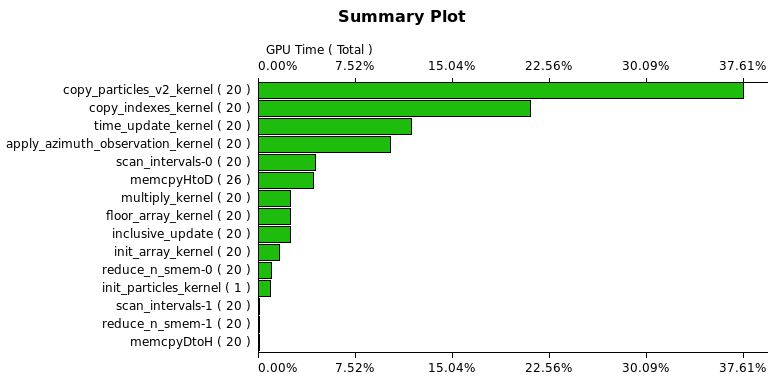
\includegraphics[width=0.7\textwidth]{data/profile_cuda_version2_pic1.png}
\caption{CUDA Visual Profiler Version 2 Results}
\label{profiler2}
\end{figure}

\subsubsection{Third Resampling Implementation}
The third resampling algorithm optimization was based on the observation that once the copy-from indexes had been stored in the weight array at the copy-to index, the weight array was equivalent to the gather map used in the thrust::gather algorithm. Gather copies items from a source array \(s[i]\) into a destination array \(d[i]\) using a map array \(m[i]\) such that \(s[i]=d[m[i]]\).\cite{thrust}

Surprisingly, especially given the amazing efficiency of thrust's reduction and scan algorithms, thrust::gather provided no speedup over my custom implementation from Section \ref{resamplesection2}. The inefficiency of the inherently uncoalesced nature of the memory access pattern most likely overwhelms any subtle performance tweaks that thrust::gather provides.

\subsection{Parallel Reduction}
The resampling calculations in Equation \ref{resample1} and \ref{resample2} require calculating the sum and cumulative sum of an array of weights. The thrust library provides prewritten parallel algorithms for common CUDA tasks, including parallel reduction.\cite{thrust}

However, before using thrust, a custom parallel array summation implementation was written based on the NVIDIA white paper on the subject included in the CUDA SDK.\cite{oprc} The core of this summation algorithm is a CUDA kernel which uses shared memory to calculate partial summations for each block.

Within each block, global memory values are copied to shared memory and a simple fan-in reduction is performed. As Figure \ref{sum1} indicates, theads add their partial sums together in a tree pattern until a single partial sum for the entire block remains. Each iteration is synchronized using \verb!__syncthreads()!.

\begin{figure}
\centering
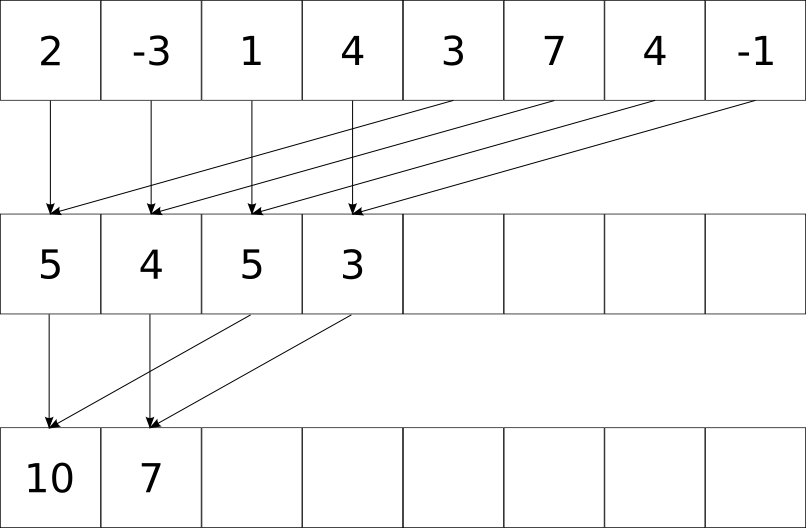
\includegraphics[width=0.7\textwidth]{data/summation.png}
\caption{Inner-block Reduction In Shared Memory Example}
\label{sum1}
\end{figure}


However, the loop construct that controls this iteration is expensive, as are the \verb!__syncthreads()! calls. Fortunately, because CUDA threads are grouped into \emph{warps} of 32 threads which execute commands simultaneously, substantial additional savings are possible once the number of partial sums in shared memory drops below 32. By stopping the reduction iteration and unrolling the final iterations, we can avoid synchronization for the iterations where all the summations are occurring within a single warp.

As each block completes its parallel summation, it writes its sum to an array in global memory. Thus, after the first iteration, global memory will contain one partial sum for each block. To sum these values, the kernel is called iteratively until fewer partial sums remain than the number of threads in a single block. At this point, the kernel is called one last time with a single block which writes the final overall sum to global memory.

\begin{figure}
\centering
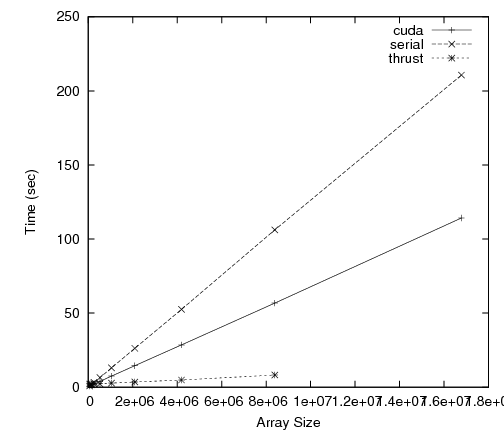
\includegraphics[width=0.7\textwidth]{data/summation_plot.png}
\caption{Array Summation Algorithm Performance}
\label{summation_plot}
\end{figure}

However, as Figure \ref{summation_plot} indicates, writing complex parallel algorithms efficiently is very difficult in CUDA. For the largest arrays tested, the custom CUDA implementation was only about twice as fast as the serial implementation whereas the thrust implementation was 12.9 times faster. These results highlight CUDA's sensitivity to subtle factors like uncoalesced memory access, shared memory bank conflicts (threads from multiple warps accessing the same sections of shared memory), and expensive gpu operations which can have significant impact on performance.\cite{bestprac}

\subsection{Random Number Generation}
Particle filter tracking is a stochastic process: as particles are time updated, they maneuver randomly according to their motion model; as particles are resampled, their replacements are randomly perturbed copies of existing particles. Thus, performing particle filter tracking using CUDA required generating random numbers efficiently on the GPU.

The thrust library provides random number generation capabilities and the CUDA SDK provides a parallel MersenneTwister example. However, the random number generator implementation used for this problem is a much simpler custom written linear congruential generator which relies on independent seeds stored for each particle. This approach is attractive because it is theoretically very fast and requires very little state, allowing each particle to generate its own independent stream of random values.

\begin{equation}\label{lcgeq1}
X_{n+1}=(aX_{n}+c \mod m)
\end{equation}

With properly chosen \(a\), \(c\) and \(m\) values linear congruential generator can provide sufficiently random values for particle filtering.\cite{lcg} The values used are those used by the java.util.Random class.

The recurrence relation in Equation \ref{lcgeq1} relies on the modulus operator, which is extremely slow on NVIDA hardware.\cite{oprc} However, this recurrence can be rewritten using the much faster shift and bitwise mask operations, avoiding the significant modulus performance hit.

\subsection{Effective Particle Count}
When resampling is performed after each observation, every particle always has an equal weight and therefore an equal chance of representing the true target state. However, resampling every iteration is not necessary.

Formula \ref{epc} calculates the effective particle count \(N_{eff}\) from a weight array \(w_{i}\).\cite{pf} This formula is best understood by considering two extreme cases. When all particles have the same weight (like after resampling is performed), we would expect the effective particle count \(N_{eff}\) to equal the actual particle count \(n\). In this case each normalized paricle weight \(\overline{w}_{i}\) will equal \(\frac{1}{n}\). Thus, \( \sum_{i=1}^{n} \overline{w}_{i}^2 \) will equal \(\frac{n}{n^{2}}\) and \(n_{eff}\) equals \(n\) as expected.

Now consider the case where one particle has weight 1 and all other particles have weight 0. In this case we expect the effective particle count to be 1 and it is trivial to show that this is indeed the case.

Because resampling is the slowest portion of the parallel particle filter code, as discussed in Section \ref{Resampling}, it makes sense to minimize the number of times it must be performed. The effective particle count metric provides a way to make that determination. Every iteration the effective particle count can be calculated relatively cheaply, and resampling can be performed only when the effective particle count falls below a given threshold.

\[\overline{w}_{i} = \frac{w_{i}}{\sum_{i=1}^{n} w_{i}}\]
\begin{equation}\label{epc}
N_{eff} = \frac{1}{\sum_{i=1}^{n} \overline{w}_{i}^2}
\end{equation}

\section{Performance}
The peak performance improvement using CUDA over the serial implementation was approximately 20 times. While this is nowhere near the theoretical performance gains which CUDA can achieve, it is respectable given the inherently uncoalesed nature of the memory accesses which the resampling strategy performs.

Figure \ref{final_timing1} displays a log-log plot of the overall execution time for the serial implementation and the CUDA implementation at various stages of optimization. Note that the CUDA timing results stop at problem sizes smaller than the serial results because of memory constraints on the Quadro FX 1700M GPU used to run the timing tests.

Both the serial and CUDA implementations scale roughly linearly with particle count. This makes intuitive sense because most operations are independent of other particles. The parts of the algorithm that do depend on other particles, like summation and cumulative summation, are performed once for all particles and scale linearly in time complexity with particle count.

The speedup factors in Figure \ref{final_timing2} achieved by the version 1, version 2, and version 2 using EPC all increase with problem size. This makes sense because GPUs do not have cached memory hierarchies to preload data, they rely on data parallelism instead of caching to hide memory latency. With smaller problem sets there are fewer blocks which reduces the ability of the GPU to swap out blocks that are stalled waiting for memory access.

It should be noted, however, that the CUDA version two test using EPC to determine when resampling is needed is not a completely fair comparison. Its speedup factor was calculated compared to a serial problem with the same particle count. However, without resampling every iteration the results will be less accurate than a serial implementation with the same particle count (although quantifying exactly how much less accurate is a difficult problem beyond the scope of this paper).

\begin{figure}
\centering
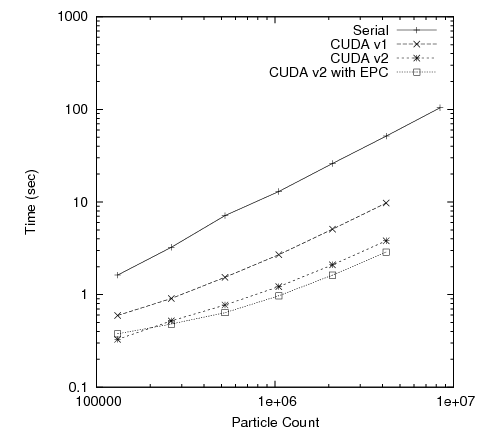
\includegraphics[width=0.7\textwidth]{data/timing_results.png}
\caption{Timing Results with 40 Observations and Variable Particle Count}
\label{final_timing1}
\end{figure}

\begin{figure}
\centering
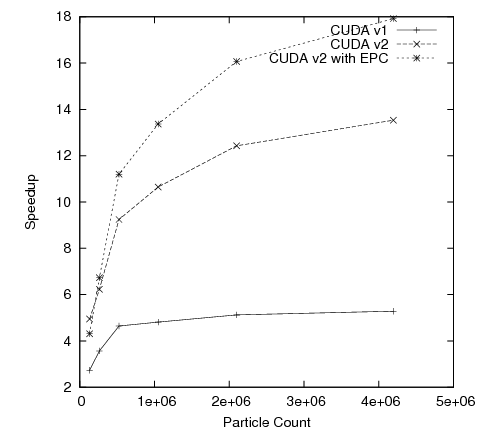
\includegraphics[width=0.7\textwidth]{data/timing_results_speedup.png}
\caption{CUDA Speedup Results with 40 Observations and Variable Particle Count}
\label{final_timing2}
\end{figure}

\begin{thebibliography}{9}

\bibitem{cpl}
  Brian W. Kernighan and Dennis M. Ritchie,
  \emph{The C Programming Language},
  Prentice Hall PTR, New Jersey,
  2009.

\bibitem{bmtt}
  Stone, Barlow, and Corwin,
  \emph{Bayesian Multiple Target Tracking},
  Artech House, Boston,
  1999.

\bibitem{oprc}
   Harris, Mark,
   \emph{Optimizing Parallel Reduction in CUDA},
   NVIDIA Developer Technology \\
   http://developer.download.nvidia.com/compute/cuda/sdk/website/samples.html

\bibitem{tutorial1}
   Volume I: Introduction to CUDA Programming \\
   http://www.nvidia.com/docs/IO/47904/VolumeI.pdf

\bibitem{bestprac}
   CUDA Best Practices Guide -- CUDA 2.2\\
   http://developer.download.nvidia.com/compute/cuda/2\_3/\\
   toolkit/docs/NVIDIA\_CUDA\_BestPracticesGuide\_2.3.pdf

\bibitem{thrust}
   Thrust C++ Template Library for CUDA \\
   http://code.google.com/p/thrust/

\bibitem{lcg}
   Linear Congruential Generator \\
   http://en.wikipedia.org/wiki/Linear\_congruential\_generator

\bibitem{pf}
   Particle Filter \\
   http://en.wikipedia.org/wiki/Particle\_filter

\end{thebibliography}

\end{document}
